\documentclass[12pt,letterpaper]{report}
\usepackage{natbib}
\usepackage{geometry}
\usepackage{fancyhdr}
\usepackage{afterpage}
\usepackage{graphicx}
\usepackage{amsmath,amssymb,amsbsy}
\usepackage{dcolumn,array}
\usepackage{tocloft}
\usepackage{asudis}
\usepackage[pageanchor=true,plainpages=false,pdfpagelabels,bookmarks,bookmarksnumbered]{hyperref}

\begin{document}
%-----------------------front matter
\pagenumbering{roman}
\title{Your Title Goes Here}
\author{Your name}
\degreeName{Doctor of Philosophy}
\paperType{Dissertation}
\defensemonth{Some month}
\defenseyear{Some year}
\gradmonth{Graduation month}
\gradyear{Graduation year}
\chair{Your chair}
\memberOne{Your first member}
\memberTwo{Your second member}
\memberThree{Your third member}
\memberFour{Your fourth member}

\maketitle
\doublespace
\begin{abstract}


Soft robots currently rely on additional hardware such as pumps,  high voltage supplies,  light generation sources, and magnetic field generators for their operation. These components resist miniaturization; thus embedding them into small-scale soft robots is challenging.  This limits their applications where the system needs to be untethered, especially in hyper-redundant mobile robots where a high number of actuators are needed. This dissertation aims at addressing some of the challenges associated with creating miniature, untethered soft robots that can function without any attachment to external power supplies or receiving any control signals from outside sources. This goal is accomplished by introducing a soft active material and a manufacturing method that together, facilitate the miniaturization of soft robots and effectively supports their autonomous, mobile operation without any connection to outside equipment or human intervention. 

The soft active material presented here is a hydrogel based on a polymer called poly(N-isopropylacrylamide) (PNIPAAm). This hydrogel responds to changes in the temperature and responds by expanding or contracting. Volumetric change is a result of water transport to and out of the porous structure of the hydrogel. The PNIPAAm chains switch from hydrophilic to hydrophobic when the temperature rises above a transition temperature; thus water is forced out from the polymer network resulting in the collapse of the network and a reduction of volume. A major challenge regarding PNIPAAm-based hydrogels is their slow response which has historically made them unsuitable for robotic applications. This challenge is addressed by introducing a mixed-solvent photo-polymerization technique that alters the pore structure of the hydrogel and facilitates the water transport and thus the rate of volume change. Using this technique, the re-swelling response time of hydrogels is reduced to 2.4 min--over 25 times faster than hydrogels demonstrated previously. The mixed-solvent method also provides a means of tuning the material properties of hydrogels including their response rate and Young's modulus by controlling the solvent ratio. The one-step photo-polymerization using UV light is performed in under 15 sec, which is a significant improvement over thermo-polymerization, which takes anywhere between a few minutes to several hours. Photopolymerization is key towards simplifying recipes, improving access to these techniques, and making them tractable for iterative design processes.

To address the challenges associated with manufacturing, a new category of soft actuators called soft voxel actuators (SVAs) is presented. SVAs are active voxels (volumetric pixels) made using stimuli-responsive hydrogels. In designing SVAs, the analogy between electrical activation of muscle tissue by the nervous system in animals is used: SVAs are actuated by electrical currents through  Joule heating.  SVAs weighing only  100 mg require small footprint microcontrollers for their operation which can be embedded in the robotic system. SVAs can be considered as building blocks assembled to form complex robots which can perform tasks that require a high number of degrees of freedom (DOF). The advantages of hydrogel-based SVAs are demonstrated through different robotic platforms namely a  hyper-redundant manipulator with 16 SVAs, an untethered miniature robot for mobile underwater applications using 8 SVAs, and a gripper using 32 SVAs.


\end{abstract}
\dedicationpage{}
{Enter your acknowledgement text here}
\tableofcontents
% This puts the word "Page" right justified above everything else.
\addtocontents{toc}{~\hfill Page\par}
% Asking LaTeX for a new page here guarantees that the LOF is on a separate page
% after the TOC ends.
\newpage
% Making the LOT and LOF "parts" rather than chapters gets them indented at
% level -1 according to the chart: top of page 4 of the document at
% ftp://tug.ctan.org/pub/tex-archive/macros/latex/contrib/tocloft/tocloft.pdf
\addcontentsline{toc}{part}{LIST OF TABLES}
\renewcommand{\cftlabel}{Table}
\listoftables
% This gets the headers for the LOT right on the first page.  Subsequent pages
% are handled by the fancyhdr code in the asudis.sty file.
\addtocontents{lot}{Table~\hfill Page \par}
\newpage
\addcontentsline{toc}{part}{LIST OF FIGURES}
\addtocontents{toc}{CHAPTER \par}
\renewcommand{\cftlabel}{Figure}
% This gets the headers for the LOF right on the first page.  Subsequent pages
% are handled by the fancyhdr code in the asudis.sty file.
\addtocontents{lof}{Figure~\hfill Page \par}
\listoffigures
%-----------------------body
\doublespace
\pagenumbering{arabic}
\chapter{INTRODUCTION}
\section{Section1}
\section{Section2}
\chapter{A NOVEL STIMLUI-RESPONSIVE HYDROGEL RECIPE FOR SOFT ROBOTICS: SYNTHESIS AND CHARACTERIZATION}
discuss different actuator technologies
\section{Stimuli-responsive Hydrogels}
Stimuli-responsive Hydrogels also known as smart hydrogels, have attracted great interest in many different fields, such as drug delivery \citesuperscript{Annabi2014,Stuart2010}, microfluidics \cite{DEramo2018a,Goy2019}, and soft robotics \citesuperscript{Banerjee2018}, owing to their large and reversible volume changes in response to a broad range of stimuli without using any additional sensors and actuators. This feature helps reduce the size of devices made of smart hydrogels. 
Stimuli-responsive, soft materials have shown promise in solving some of these challenges \cite{steele2018stimuli, stuart2010emerging,white2013advances}. The changes in the stress/strain distribution in these materials in reaction to variations in pH, temperature, electric field, magnetic field, and light results in motions such as bending, twisting, or elongation. Practical soft robotic applications, ranging from basic bending and shortening primitives to complex reconfigurations, all require time-varying and local deformations of bulk hydrogels in order to approach the dexterity of 
% better mimic  the functions of 
soft organisms in performing tasks such as grasping and manipulation \citesuperscript{Ionov2014, Erol2019}.
However, the responsive volume change of smart hydrogels is typically uniform.
Two main approaches have been adopted by researchers to achieve nonuniform spatiotemporal deformation in hydrogels \citesuperscript{Ionov2014}. In the first approach, heterogeneous structures in the shape of sheets and rods are fabricated by patterning material domains using manufacturing techniques such as micro- and meso-patterning \citesuperscript{Zhou2018b,Klein2007,Kim2012,Ma2016a,Erb2013,Huang2017} and 3D printing \citesuperscript{Zheng2018}. Differing swelling properties of neighboring domains upon stimulation results in nonuniform strain fields in these structures, causing them to transform into a variety of complex shapes like coils and conical helices \citesuperscript{Wu2013,Liu2016}.
The range of compatible materials available for each domain, however, is often limited by practical fabrication constraints, such as ink viscosity for 3D printing \citesuperscript{Zheng2018}. Moreover, the geometry and material selected for each domain determine the shape transformations; these features cannot be changed after manufacturing, making on-demand reconfiguration infeasible.\\

The second approach towards achieving nonuniform spatiotemporal deformations uses an inhomogeneous or time-varying stimulus, such as patterns of structured light \citesuperscript{Palagi2016a}, local irradiation by near-infrared light \citesuperscript{Mourran2017}, or localized electric fields \citesuperscript{Choi2020}. In these methods, the hydrogel material itself is typically homogeneous, but the stimulus intensity varies across different regions, causing localized and time-varying deformations. These techniques, while suitable for on-demand shape reconfiguration, often require bulky external equipment, ultimately leading to challenges in mobile robot applications.\\
%applications. Hence, in these approaches, the limited design flexibility and spatiotemporal re-programmability have remained key challenges for realizing complex motion in soft robotic tasks.

Nature has adopted a hierarchical approach in addressing these challenges by using motor units as building blocks for heterogeneous muscle tissue demonstrating complex spatiotemporally reprogrammable deformations  \citesuperscript{frontera2015skeletal, drost2003spatial}. A motor unit consists of a motor neuron and the muscle fibers innervated by its axonal terminals \citesuperscript{buchthal1980motor}.
% , as shown in \firstsubfigref{fig:1}{A, right}.  
% it is a  in biological systems such as octopuses, caterpillars, and worms 
It behaves as a stimuli-responsive building block, producing unidirectional deformation in response to electrical stimulus from the central nervous system (CNS). 
% or peripheral nervous system (PNS) 
 The variations in orientation \citesuperscript{KIER1985}  and response rate \citesuperscript{Kier1992} of muscle fibers create the structural heterogeneity \citesuperscript{Liu2017b} required for nonuniform hard-coded deformations; the on-demand control over location and intensity of the electrical stimulus provides the spatiotemporal reprogrammability \citesuperscript{Hanassy,Kazakidi2015,Richter2015}.\\
 
Virtual voxels have been used for decades as building blocks to represent shapes in 3-D space for computer graphics applications \citesuperscript{Yagel1993}.
% are shown to have the potential as building blocks for simulating and manufacturing heterogeneous structures. 
More recently, voxel-based simulations have been used to predict bulk material properties of structures -- including structures made of smart hydrogels -- by controlling the material properties of individual virtual voxels \citesuperscript{Hiller2010,Oxman2011,Sossou2019}. Virtual voxels have also been utilized to simulate heterogeneous structures with robotic functions \citesuperscript{Cheney2014}. 
% bulk hydrogels rk{\citesuperscript{Yuan2017,Cheney2014}} and 
However, physical realization of voxels as building blocks have been limited to passive and often rigid materials, and are used in conjunction with additive manufacturing processes to increase their throughput \citesuperscript{Hiller2009}. One recent work has used voxel-based computer simulations to optimize the distribution of active and passive materials in a structure for achieving different goals and the resulting mechanisms are physically realized using cardiomyocytes from a frog as building blocks for creating responsive structures\citesuperscript{Kriegman2020}.\\

Inspired by nature's approach for achieving on-demand spatiotemporal deformations in muscle tissue, we introduce addressable and tunable building blocks that can be assembled to create heterogeneous hydrogel structures with \textit{hard-coded} or \textit{reprogrammable} shape change. These building blocks, herein referred to as soft voxel actuators (SVAs), are shown in \firstsubfigref{fig:1}{A}, left. The SVA units, consisting of a responsive hydrogel material and corresponding electrical connections, are inspired by the motor units of muscle tissue (\subfigref{fig:1}{A}, right).
% , which consist of a motor neuron and the responsive muscle fibers associated with it. 
The deformation of SVA units as a result of an electrical stimulus from a microcontroller unit (MCU) is analogous to the contraction of muscle fiber units in response to stimuli from the central nervous system (CNS).
% as seen in \firstsubfigref{fig:1}{A}, left. 
The selection of electrical stimuli as opposed to other types of stimuli is advantageous, since it enables addressing SVAs directly by small-footprint microcontrollers without the need for bulky equipment or human intervention. \citesuperscript{Yu2013}.\\




However, the equipment needed to create variable stimuli such as structured light \cite{palagi2016structured} or magnetic field \cite{Kim2018} are still bulky.  
Temperature responsive hydrogels, by contrast, can be stimulated electrically using Joule heating \cite{yu2013electronically}. The electrical stimulation can be confined to small regions making it possible to create more precise motions \cite{richter2009optoelectrothermic}. 

We have previously reported solving some of the challenges associated with temperature responsive poly(N-isopropylacrylamide) (PNIPAAm) based hydrogels such as their slow response and tuning their mechanical properties. We have also introduced blocks called soft voxel actuators (SVAs), which are electrically activated by Joule heaters \cite{khodambashi2021heterogeneous}. 
In this communication, we demonstrate how SVAs support the development of soft robots which are miniature and untethered --two key characteristics that are challenging to realize with pneumatic soft actuators. We introduce a miniature completely untethered robot for underwater applications which weighs only 20\,g including battery and electronics as shown in Fig.~\ref{fig:concept}. We also demonstrate the use of SVAs to build a miniature continuum manipulator with hyper-redundant DOFs as shown in Fig.~\ref{fig:treajectory}A. This manipulator is 10$\times$ 40 $\times$ 4.5\,mm$^3$ and has 16 actuators. 

material characterization
sem images
mechanisms behind response rate
detailed literature review
\section{Section1}
\section{Section2}
\chapter{MATERIAL CHARACTERIZATION}
\section{Section1}
\section{Section2}
\chapter{Miniature Hyper-redundant Soft Manipulator}
manufacturing
characterization
\section{Section1}
\section{Section2}
\chapter{Miniature Untethered Underwater Walking Robot}
Manufacturing 
Characterization
\section{Section1}
\section{Section2}
\chapter{Conclusion}
what is heterogeineity?
detailed literature survey
soft voxel actuators
\section{Section1}
\section{Section2}
%-----------------------back matter
{\singlespace
% Making the references a "part" rather than a chapter gets it indented at
% level -1 according to the chart: top of page 4 of the document at
% ftp://tug.ctan.org/pub/tex-archive/macros/latex/contrib/tocloft/tocloft.pdf
\addcontentsline{toc}{part}{REFERENCES}
\bibliographystyle{asudis}
\bibliography{dis}}
\renewcommand{\chaptername}{APPENDIX}
\addtocontents{toc}{APPENDIX \par}
\appendix
\chapter{RAW DATA}

\chapter{Curriculum Vitae}
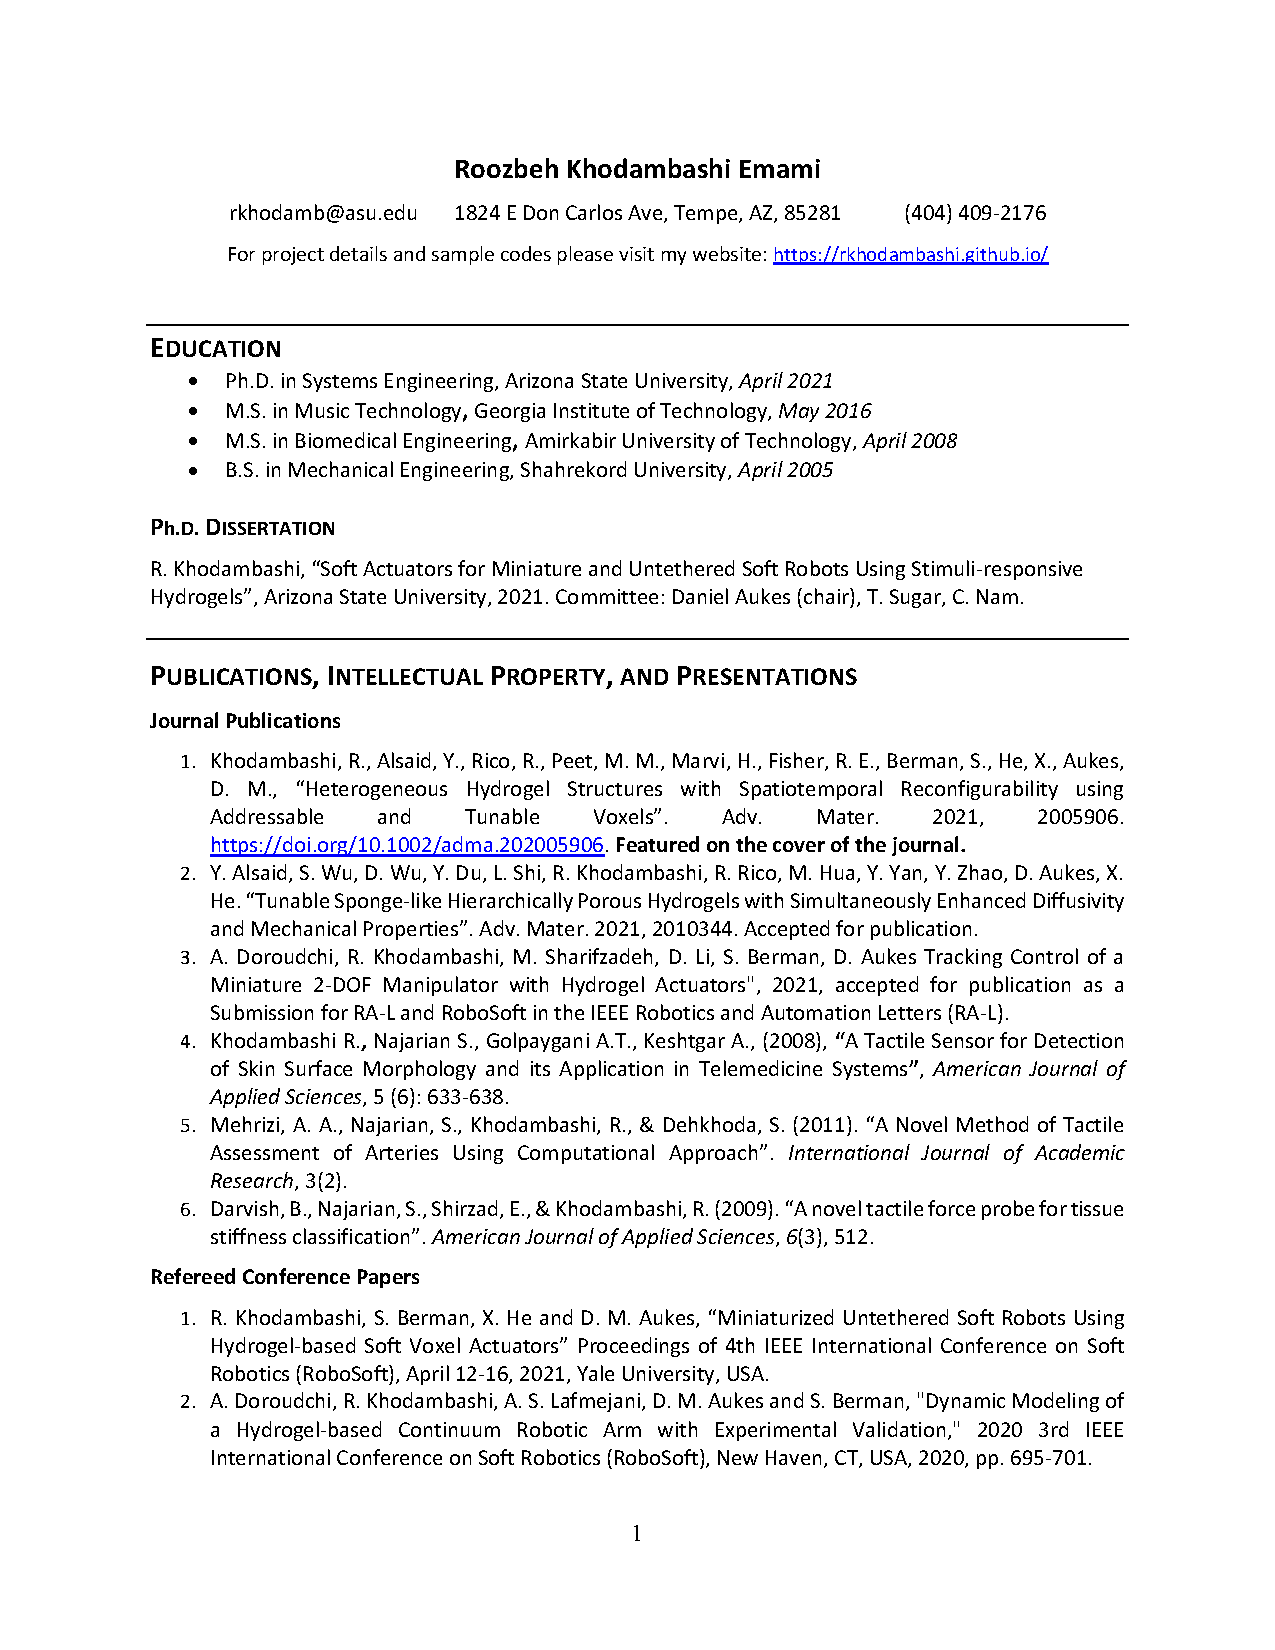
\includepdf[pages=-,pagecommand={},width=1.3\textwidth]{CV.pdf}


\end{document}
